\chapter{Introduction}

Financial institutions make decisions on whether to buy or sell assets based on various reasons, including: customer requests, fundamental analysis\cite{fundamental-analysis}, technical analysis\cite{technical-analysis}, top-down investing\cite{td-investing}, bottom-up investing\cite{bu-investing} and many more. 
The high-level trading strategies oftentimes define the purpose of their business and how the institution positions itself in the financial markets and, if existent, towards its customers. 
Regardless of the high-level trading strategy that is being applied, the invariable outcome is the decision to buy or sell assets.
This work aims to make a step towards answering the non-trivial question on how to optimize a buy or sell of an asset on a stock exchange with the use of reinforcement learning techniques.
The following sections will elaborate this problem in detail and state the research objectives of this work. 
We then list the contributions made to the scientific community throughout this work, followed by a brief overview of the structure of this report.

\section{Problem Statement}

We are concerned about which are traded at stock exchanges.
Regarding stock exchanges there is little consensus as to when corporate stock was first traded; some argue that the exchange, in the form as we know it today, dates as far back as 1531, when the East Indian Company stock was traded in Antwerp\cite{stock-exchange}.
Modern financial markets such as the London Stock exchange (LSE), the New York Stock Exchange (NYSE) but also the numerous cryptocurrency exchanges which appeared suddenly in the last few year, all rely on the same very same principles as back then.
Every participant is either willing to buy or sell a given amount of an asset to, respectively for, a certain price.

When in the late '90s the regulatories started to let traders reach into the market using electronic communications networks (ECNs), a new era arose \cite{patterson2012dark}.
High frequency traders (HFT) and algorithmic traders suddenly gained advantage over the traders who placed their orders manually.
Nowadays anything else than trading trough electronic channels would be unthinkable.
This certainly reduced the advantages some parties have over others, however, a certain gap still remains.
Investors without fibre access to the exchange and supporting algorithms will likely take a small initial loss into account when buying or selling assets -- and might not even be aware of it.

\begin{figure}[H]
    \centering
    \makebox[\linewidth]{
        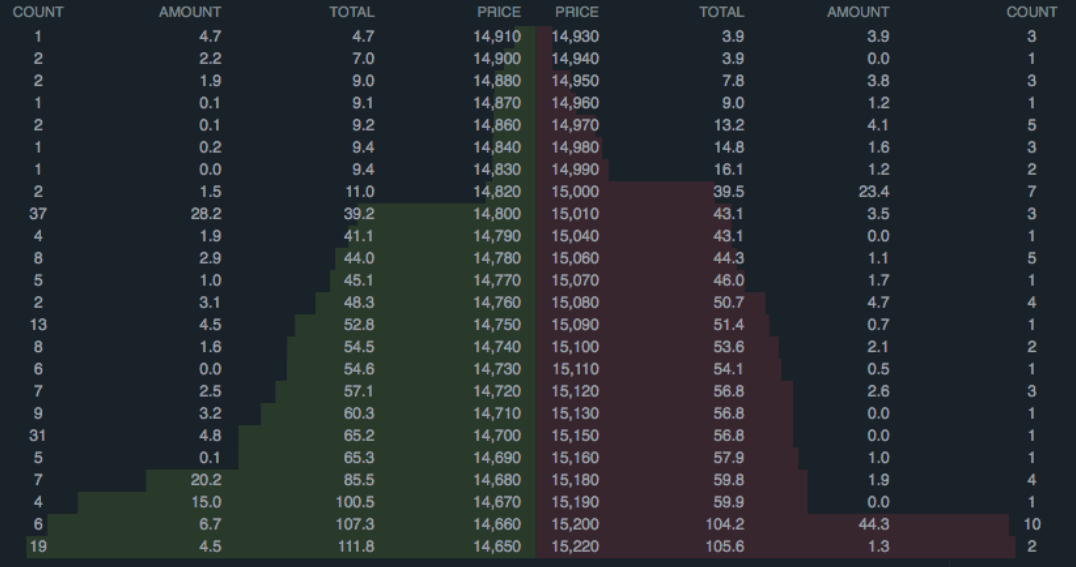
\includegraphics[width=\linewidth]{orderbook-gdax.png}
    }
    \caption{Order book snapshot: https://www.bitfinex.com/t/BTC:USD}
    \label{fit:intro-orderbook}
\end{figure}

Figure \ref{fit:intro-orderbook} shows a snapshot taken at some time $t$ from the trading pair Bitcoin (BTC) versus US dollar (USD) taken at the Bitfinex\footnote{https://www.bitfinex.com} cryptocurrency exchange.
The order book shows two sides, the parties who are willing to buy on the left and the parties who are willing to sell on the right.
The columns indicate the number of buyers and sellers (\textit{count}) who are willing to buy, respectively sell, a certain \textit{amount} for a given \textit{price}.
The column \textit{total} is simply the cumulative sum of the amount, or volume, on each side.
The two sides are separated by the \textit{spread}. 
In this particular case, the current best \textit{bid} price at which someone is willing to buy, is \$14,910.00 and the best ask-price at which someone is willing to sell, is \$14,930.00. 
Therefore, the spread is currently \$20.00 wide.
\\
\\
Suppose we want to buy 1.0 BTC.
In simplified terms, there are essentially two possible ways to do so:
\begin{enumerate}
    \item Buy $i$ shares (1.0) right away for \$14,930.00 from a seller. We submit a \textit{market} order.
    \item State a price for which we are willing to to buy $i$ shares (1.0) at price $p$, for example at \$14'910.00, and wait until someone is willing to sell for this price. We submit a \textit{limit} order.
\end{enumerate}

Both types of orders come with their advantages and disadvantages.
A market order ensures that we will be able to acquire the stated amount of shares immediately for \$14'930.00, provided that no one else is ahead of us or the seller cancels his/her listing. 
In this case we are automatically willing to pay for the next available best price.
However, we do pay a premium compared to the limit order.

With a limit order the exchange guarantees that we will pay \$14'910.00 or less.
However, this comes with the risk that we will never be able to buy if nobody is going to sell at the mentioned price, which will force us to buy for a higher price within a specified time horizon $H$.
Thus, we pay an \textit{opportunity cost}.
Likewise, if a seller realizes that we are about to buy for price $p$ at which is was willing to sell, he then could \textit{cancel} his offer as his incentive is to sell for a higher price.
Perhaps this has been his/her intention to only post an offer but withdrawal as soon as a counter-offer will be listed that is close to his/her price.
This method is known as \textit{quote stuffing}.
\\
\\
Clearly, posting an order is not as trivial as one would think.
Nevertheless, the prices for some financial products, including cryptocurrencies, are very volatile such that it is likely to be able to buy for less than what is offered at the mentioned time $t$.
Thus, placing orders \textit{deeper} in the book and wait could be beneficial.
According to Guo et. al. \cite{guo2013optimal} algorithmic trading is based on two different time scales: \textit{order execution} concerns about optimally slicing big orders into smaller ones in order to minimize the \textit{price impact}, that is, on a daily or weekly basis.
\textit{Order placement} on the other hand concerns about optimally placing orders within ten to hundred seconds. 
In this thesis we are concerned about the latter, which conforms the context of the problem: at which price $p$ should one attempt to buy or sell $i$ shares of an asset and what are the factors that might interfere with our intention to do so, within a time horizon $H$ of 100 seconds.
The fact that reinforcement learning does not require any supervision and instead learns by maximizing rewards, makes this technique unarguably suitable to work within this context.

\section{Research objectives}

This work should extend on the findings of Kearns et. al. \cite{nevmyvaka2006reinforcement} with the aim to understand and learn from the outcome of limit order placement in a given market.
With this knowledge we should build a reinforcement learner that can act as an intelligent trader and places limit orders such that the outcome is the buy or sell of an asset to a favourable price.
Therefore we shall build a framework that let us simulate and understand the outcome of order placement and more importantly allows to build reinforcement learning tools on top.
We further have to reason about what features can be derived from an order book and if there are any patterns that can be detected, such that this information could contribute to the learning process.
Lastly, we shall lay a focus on deep reinforcement learning techniques as this has had great success on learning to play video games \cite{mnih2013playing} based on a history of pixel inputs, but has never been applied to the optimal order placement problem.

Hence, the main objective of this research can be formulated in one sentence: \begin{quote}
    How should one design a reinforcement learning environment and construct features, which are derived from a limit order book, in order to optimize on the non-trivial problem of limit order placement, and what are the limitations thereof?".
\end{quote}

\section{Contributions}

This thesis makes use of concepts from various research communities in order to work on the above mentioned objectives.
The particular contributions made throughout the project are:
\begin{itemize}
    \item \textit{Information retrieval} techniques are provided in order to collect and process financial data sets.
    \item \textit{Software engineering} contributions to a simulation of a rudimentary stock exchange and a set of tools that can be used for data science purposes.
    \item \textit{Reinforcement learning} is the main contribution. Various approaches are developed and investigated related to \textit{order placement} and \textit{market making}.
\end{itemize}


\section{Document structure}

We first provide in Chapter \ref{chap:preliminaries} background information to the reader concerning the components of a stock exchange and the fundamentals of the closely related time series.
We further make the reader familiar with (Deep) Reinforcement Learning.
In Chapter \ref{chap:related-work} we elaborate on the behaviour of order execution followed by approaches of both statistical and machine learning nature.
Chapter \ref{chap:data} explains the process of data collection and its preparation which was done prior its use in the following chapters.
Namely, Chapter \ref{chap:setup} explains the experimental setup of the Reinforcement Learning environments, the agents and the features being processed and used.
In Chapter \ref{chap:analysis} we then analyze the data and proceed execution placement with various techniques, including the reasoning of our findings.
Finally, Chapter \ref{chap:conclusion} formulates a conclusion of our findings and states a future research direction.
